\documentclass[a4paper]{article}
\usepackage[fontset=fandol]{ctex}
\usepackage{amsmath,amssymb}
\usepackage{graphicx}
\usepackage[margin=2.35cm]{geometry}
\usepackage[most]{tcolorbox}
\usepackage{etoolbox}
\usepackage{listings}
\usepackage{hyperref}
\usepackage{booktabs}
\usepackage{array}
\usepackage{float}
\usepackage{xcolor}

\definecolor{kbBack}{HTML}{F2F6FA}\definecolor{kbFrame}{HTML}{9DB4CC}\definecolor{kbTitle}{HTML}{52708F}
\definecolor{ibBack}{HTML}{FBF5E7}\definecolor{ibFrame}{HTML}{C9A961}\definecolor{ibTitle}{HTML}{7D5F1E}
\definecolor{wbBack}{HTML}{FCF2F0}\definecolor{wbFrame}{HTML}{D6A096}\definecolor{wbTitle}{HTML}{9E4F43}
\definecolor{dbBack}{HTML}{F4F7F3}\definecolor{dbFrame}{HTML}{AEC2AC}\definecolor{dbTitle}{HTML}{5F7F64}

\tcbset{softbox/.style={enhanced,breakable,boxrule=0.8pt,arc=2pt,left=3mm,right=3mm,top=2mm,bottom=2mm,coltitle=white,fonttitle=\bfseries,toptitle=0.6mm,bottomtitle=0.6mm}}
\newtcolorbox{knowledgebox}[1]{softbox,colback=kbBack,colframe=kbFrame,colbacktitle=kbTitle,title=#1}
\newtcolorbox{importantbox}[1]{softbox,colback=ibBack,colframe=ibFrame,colbacktitle=ibTitle,title=#1}
\newtcolorbox{warningbox}[1]{softbox,colback=wbBack,colframe=wbFrame,colbacktitle=wbTitle,title=#1}
\newtcolorbox{dialoguebox}[1]{softbox,colback=dbBack,colframe=dbFrame,colbacktitle=dbTitle,title=#1}

\lstset{language=Python,basicstyle=\ttfamily\small,keywordstyle=\color{blue!65!black},stringstyle=\color{red!60!black},commentstyle=\color{green!45!black},breaklines=true,frame=single,numbers=left,numberstyle=\tiny\color{gray},captionpos=b,extendedchars=false}
\hypersetup{colorlinks=true,linkcolor=blue!50!black,urlcolor=blue!60!black}
\setlength{\parindent}{2em}
\setlength{\parskip}{0.35em}
\setlength{\emergencystretch}{2em}
\renewcommand{\arraystretch}{1.25}

\newcommand{\makelecturetitle}{
\begin{titlepage}
\centering
\vspace*{0.8cm}
{\huge\bfseries \notetitle\par}
\vspace{0.6cm}
{\large \lecturers\par}
\vspace{0.25cm}
{\large \noteauthors\par}
\vspace{0.8cm}
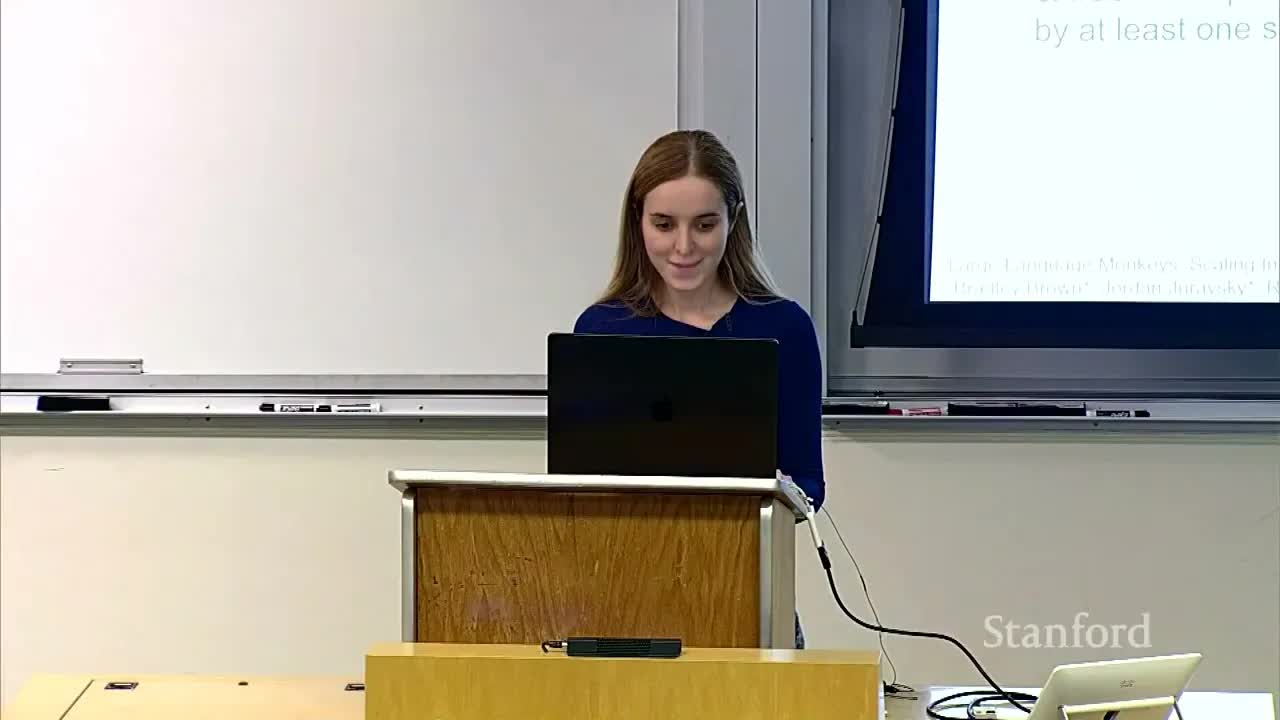
\includegraphics[width=0.86\textwidth,height=0.44\textheight,keepaspectratio]{cover.jpg}
\vfill
\begin{tcolorbox}[width=0.92\textwidth,colback=black!2!white,colframe=black!55,sharp corners]
\textbf{课程}：Stanford CS329A Self-Improving AI Agents（Autumn 2025）\par
\textbf{本讲日期}：\lecturedate\quad
\textbf{公开视频发布日期}：2026-08-03\par
\textbf{讲义制作日期}：\notedate\par
\textbf{频道 / 时长}：Stanford Online\quad / \videoduration\par
\textbf{视频链接}：\href{\videourl}{\nolinkurl{\videourl}}\par
\textbf{制作规范}：\href{https://github.com/wdkns/wdkns-skills}{wdkns/wdkns-skills}（commit \texttt{39f1a04}）与本项目质量规范
\end{tcolorbox}
\end{titlepage}
\tableofcontents
\newpage
}

\newcommand{\videofigure}[4][0.95]{
\begin{figure}[H]
\centering
\includegraphics[width=#1\textwidth]{#2}
\caption{#3\protect\footnotemark}
\end{figure}
\footnotetext{视频讲解区间：#4。}
}


\newcommand{\talkfigure}[2]{%
    \begin{figure}[H]
        \centering
        \includegraphics[width=0.95\textwidth]{#1}
        \caption{#2}
    \end{figure}%
}

\begin{document}
\begin{titlepage}
\centering
\vspace*{0.18\textheight}
{\Huge\bfseries Agent测试时计算扩展\par}
\vspace{1.6cm}

\begin{minipage}{0.86\textwidth}
\raggedright
{\Large\bfseries 相关论文\par}
\vspace{0.6em}
\large
\begin{enumerate}
    \setlength{\itemsep}{0.8em}
    \item Large Language Monkeys: Scaling Inference Compute with Repeated Sampling
    \item Scaling LLM Test-Time Compute Optimally can be More Effective than Scaling Model Parameters
    \item Archon: An Architecture Search Framework for Inference-Time Techniques
\end{enumerate}
\end{minipage}
\end{titlepage}

\begingroup
\small
\tableofcontents
\endgroup
\newpage

\section{固定模型下的推理计算}

训练阶段的 scaling law 描述训练计算量与模型性能的关系。

\textbf{在模型参数固定以后，能否通过更多采样、搜索、修订和验证，提高同一个模型的最终成功率？}

\begin{enumerate}
    \item \textbf{Large Language Monkeys}\quad 重复采样为什么呈现可预测的 scaling law？
    \item \textbf{Compute-optimal test-time scaling}\quad 并行采样和串行修订应如何分配预算？
    \item \textbf{Archon}\quad 如何自动搜索由 generator、critic、ranker、fuser 和 verifier 组成的推理架构？
\end{enumerate}

\begin{importantbox}{生成、验证与预算分配}
\textbf{生成}决定候选集能否覆盖正确解，\textbf{验证}决定能否识别正确解，\textbf{预算分配}决定有限计算能否用在收益最高的操作上。任何一个环节成为瓶颈，都会限制最终收益。
\end{importantbox}

\subsection{候选覆盖率与选择策略}

\begin{table}[H]
\centering
\begin{tabular}{p{3.1cm}p{10.5cm}}
\toprule
\textbf{指标} & \textbf{含义} \\
\midrule
pass@1 & 系统只交付一个答案时的最终准确率 \\
pass@$k$ / coverage & $k$ 个候选中至少存在一个正确答案的概率 \\
best-of-$N$ & 生成 $N$ 个候选后，由某个 verifier 选择一个答案 \\
majority@$N$ & 按答案频率投票，隐含“正确答案最常出现”的假设 \\
\bottomrule
\end{tabular}
\end{table}

增加采样首先扩大候选集。系统最终只交付一个答案，因此需要分别测量 coverage 与 pass@1。比较策略时，需要权衡候选质量、选择质量与计算成本。

\section{Large Language Monkeys：重复采样的 Scaling Law}

\subsection{生成与验证的两阶段系统}

Repeated sampling 先从同一模型独立采样多个候选，再交给 verifier 选择。代码与形式化证明尤其适合这种方法，因为单元测试、编译器和 proof checker 能提供接近确定性的自动反馈。

\talkfigure{figures/generate-verify.jpg}{多候选生成与验证构成 inference scaling 的基本流水线。}

假设问题 $i$ 的单次采样成功概率为 $p_i$，独立采样 $k$ 次的 oracle coverage 为：

$$
C_i(k)=1-(1-p_i)^k.
$$

\begin{itemize}
    \item $p_i$：模型对问题 $i$ 的单次成功概率；
    \item $k$：采样数；
    \item $C_i(k)$：候选集合至少包含一个正确解的概率。
\end{itemize}

这说明每道题自身呈指数饱和：初始采样带来最大收益，之后边际增益逐步下降。

\subsection{小模型为何能通过采样追上强模型}

只要 $p_i>0$，增加 $k$ 就能提高 coverage。实验中，较小模型通过大量采样在数学、代码和形式化证明上显著缩小与强模型单次推理的差距。

\talkfigure{figures/repeated-sampling.jpg}{重复采样在多个 reasoning benchmark 上提高了正确候选的覆盖率。}

\begin{knowledgebox}{能力被“放大”还是被“发现”}
Repeated sampling 在模型参数固定时从已有的输出分布中反复抽样。采样次数越多，越有机会抽到低概率的正确轨迹。收益来自更充分地\textbf{发现并利用模型已有的能力}。
\end{knowledgebox}

\subsection{从单题指数曲线到数据集平均幂律}

平均 coverage 随采样数的变化可以用 exponentiated power law 拟合。

$$
\bar C(k)\approx 1-\exp(-a k^b),\qquad a>0,\;0<b<1.
$$

\begin{itemize}
    \item $\bar C(k)$：数据集上的平均 coverage；
    \item $a$：与模型和任务总体难度相关的尺度参数；
    \item $b$：控制 scaling 速度的指数；
    \item $k$：推理采样预算。
\end{itemize}

\talkfigure{figures/inference-scaling-law.jpg}{平均 coverage 随采样数呈可预测的 exponentiated power law。}

单题 coverage 按 $1-(1-p_i)^k$ 指数饱和。为什么对问题取平均后会出现幂律？数据集中有大量模型偶尔才能解出的难题，它们在 $p_i$ 接近零的位置形成长尾。

\talkfigure{figures/scaling-across-models.jpg}{从小模型到大模型都观察到 inference scaling。}

\subsection{长尾是平均幂律的充分条件}

若问题成功概率在 $p\rightarrow0$ 附近具有密度

$$
f(p)\propto p^{\alpha-1},
$$

则数据集平均失败率近似为：

$$
1-\bar C(k)=\mathbb{E}_{p}[(1-p)^k]
\approx\int_{0}^{\infty} e^{-kp}p^{\alpha-1}\,dp
\propto k^{-\alpha}.
$$

\begin{itemize}
    \item $f(p)$：不同问题的单次成功概率分布；
    \item $\alpha$：靠近零点的长尾指数；
    \item $k^{-\alpha}$：随着采样预算增长而衰减的平均失败率。
\end{itemize}

\talkfigure{figures/long-tail-theorem.jpg}{大量低成功概率问题使数据集平均 pass@$k$ 呈幂律扩展。}

\begin{importantbox}{长尾决定采样收益何时饱和}
如果所有题的 $p_i$ 都较高，少量采样后就饱和；如果大量题的 $p_i$ 极低但非零，收益会延续到很大的 $k$。因此推理 scaling 的形状不仅由模型决定，也由 benchmark 难度分布决定。
\end{importantbox}

\subsection{预训练与推理的预算权衡}

如果基础模型已经偶尔能生成正确解，且 verifier 能识别这类候选，按请求增加推理计算可以提高成功率。对少量高价值请求，这可能比训练和部署更大的模型更经济。

\talkfigure{figures/compute-allocation.jpg}{训练大模型后单次推理，或用适中规模的模型按请求分配推理预算。}

不同规模的模型都表现出 oracle coverage 随采样预算增长的规律。覆盖率能转化为多少最终准确率，取决于 verifier 能否识别候选集中的正确解。

\section{Generation--Verification Gap}

\subsection{Oracle coverage 是固定候选集下的准确率上界}

只要候选集中有正确答案，知道 ground truth 的 oracle verifier 就能选中它。实际选择器通常使用多数投票、reward model 或 LLM judge，最终准确率可能远低于这个上界。

\talkfigure{figures/verification-gap.jpg}{常见选择器的实际准确率低于候选集合的 oracle coverage。}

两者的差值是 generation--verification gap。

$$
G(k)=C_{\mathrm{oracle}}(k)-A_{\mathrm{selector}}(k),
$$

\begin{itemize}
    \item $C_{\mathrm{oracle}}(k)$：候选集合中存在正确答案的比例；
    \item $A_{\mathrm{selector}}(k)$：真实选择器交付正确答案的比例；
    \item $G(k)$：generation--verification gap。
\end{itemize}

\subsection{为什么 majority vote 会失败}

多数投票按出现频率选择答案。对困难问题，模型可能反复生成相似的错误解，正确解只偶尔出现。

\talkfigure{figures/rare-correct.jpg}{正确候选可能位于输出分布的稀有尾部。}

\begin{warningbox}{Self-consistency 依赖一个隐藏假设}
多数投票依赖正确答案比任一错误答案更常出现。如果某一种错误更常见，增加采样会让投票结果更稳定地偏向该错误。候选间的一致性反映答案出现的频率，正确性仍需验证。
\end{warningbox}

\subsection{验证器应具备什么性质}

\begin{itemize}
    \item \textbf{Soundness}\quad 拒绝明显错误的候选。
    \item \textbf{Recall}\quad 尽可能识别候选中的稀有正确解。
    \item \textbf{Calibration}\quad 评分应反映实际成功概率。
    \item \textbf{Robustness}\quad 对候选的风格、长度和表面自信保持稳健。
    \item \textbf{Cost}\quad 验证成本应显著低于重新生成或人工检查。
\end{itemize}

\begin{knowledgebox}{可验证领域的结构优势}
数学形式化证明和代码执行可把 verifier 外包给符号系统或真实环境。开放式写作、战略决策和科学假设则缺少便宜 ground truth，只能使用 learned reward model 或延迟反馈，因此更容易出现验证瓶颈。
\end{knowledgebox}

生成器变强或采样增多时，候选分布可能更复杂，选择器识别稀有正确解的难度也可能上升。验证可靠性因此制约着额外采样能带来的实际准确率提升。

\section{Compute-Optimal Test-Time Scaling}

\subsection{并行采样与串行修订}

增加 test-time compute 有两种基本方式：

\begin{itemize}
    \item \textbf{Parallel sampling}：从同一 prompt 独立生成多个候选，强调多样性；
    \item \textbf{Sequential revision}：让模型读取中间结果并修订，强调单轨迹深度。
\end{itemize}

\talkfigure{figures/parallel-sampling.jpg}{并行采样用多个独立候选扩大搜索宽度。}

并行方法易于扩展，且错误不会跨候选传播；串行方法能利用反馈逐步改进，但若早期方向错误，后续步骤可能围绕错误前提继续优化。

\subsection{Outcome Reward Model 与 Process Reward Model}

\talkfigure{figures/reward-model-types.jpg}{Outcome reward 与 process reward 提供不同粒度的搜索信号。}

\begin{itemize}
    \item \textbf{ORM}（Outcome Reward Model）：只评价最终答案；适合 best-of-$N$，信用分配粗；
    \item \textbf{PRM}（Process Reward Model）：逐步评价推理过程；可用于 beam search 和提前剪枝。
\end{itemize}

若一条轨迹包含步骤 $z_{1:T}$，PRM 可提供局部得分 $r_t=r(z_t\mid z_{<t},x)$，搜索器据此保留高潜力分支，而无需等到完整答案生成后才发现错误。

\subsection{组合搜索宽度与深度}

Compute-optimal 策略在总预算内组合并行采样和串行修订。系统可以先探索多个初始候选，再对高分候选进行多轮修订。

\talkfigure{figures/hybrid-search.jpg}{并行采样扩大宽度，revision model 增加搜索深度。}

并行采样、串行修订与验证共用预算 $B$。

$$
B=n_{\mathrm{parallel}}\cdot c_{\mathrm{sample}}
+n_{\mathrm{revise}}\cdot c_{\mathrm{revise}}
+c_{\mathrm{verify}}.
$$

\begin{itemize}
    \item $B$：单题总推理预算；
    \item $n_{\mathrm{parallel}}$：并行候选数；
    \item $n_{\mathrm{revise}}$：串行修订轮数；
    \item $c_{\mathrm{sample}},c_{\mathrm{revise}},c_{\mathrm{verify}}$：各操作成本。
\end{itemize}

\subsection{最优预算分配随问题难度变化}

\talkfigure{figures/compute-optimal-results.jpg}{在 PRM 指导下，compute-optimal search 早期收益高于纯 best-of-$N$。}

\talkfigure{figures/parallel-sequential-ratio.jpg}{简单题偏向串行修订，困难题需要一定并行探索。}

初始解的质量影响搜索宽度与深度的取舍。

\begin{itemize}
    \item 简单题通常已有接近正确的初始解，revision 能快速修正；
    \item 困难题的初始解可能落入完全错误的思路，需要并行探索不同方向；
    \item 过度串行会把预算浪费在修补不可救的轨迹；
    \item 过度并行则产生大量浅层候选，没有充分利用反馈。
\end{itemize}

\subsection{测试时 FLOPs 何时胜过预训练 FLOPs}

\talkfigure{figures/testtime-vs-pretraining.jpg}{中等难度问题常从 test-time compute 获益，而最难问题仍受基础能力限制。}

\begin{importantbox}{基础模型能力限制推理扩展}
当基础模型几乎采样不到正确轨迹时，增加搜索的收益有限。实验中，最难的问题从额外推理计算中获益很小。扩大预训练或改进训练数据更可能改善这类问题的表现。
\end{importantbox}

\subsection{在线预算分配}

在线调度需要根据问题难度、模型能力和 verifier 质量估计边际收益，据此选择继续采样、修订、验证或停止。

\section{Archon：搜索 Inference-Time Architecture}

\subsection{把推理系统视为可搜索架构}

Archon 借用神经网络的分层结构来组织 inference-time operations，再搜索各层的操作组合、顺序、模型来源和调用次数。

\talkfigure{figures/archon-framework.jpg}{Archon 根据目标 benchmark 和可用模型搜索优化后的推理架构。}

其输入包括目标任务、候选模型、可用操作和成本约束；输出是一张执行图。例如多个 generator 并行采样，critic 识别缺陷，ranker 选择候选，fuser 综合答案，再进行下一轮批评与融合。

\subsection{可组合操作}

\talkfigure{figures/archon-operations.jpg}{Archon 中常见 inference-time operation 的定义、输入、输出与成本。}

\begin{table}[H]
\centering
\small
\begin{tabular}{p{2.8cm}p{5.1cm}p{5.7cm}}
\toprule
\textbf{操作} & \textbf{功能} & \textbf{主要风险} \\
\midrule
Generator & 产生一个或多个候选 & 缺乏多样性、重复错误 \\
Critic & 指出候选缺陷与遗漏 & 批评不准确或只关注表面形式 \\
Ranker & 对候选排序 & 位置偏差、长度偏差、judge 偏差 \\
Fuser & 综合多个候选的互补部分 & 把错误也融合进去 \\
Verifier / Tests & 检查约束与正确性 & 测试覆盖不足、奖励投机 \\
\bottomrule
\end{tabular}
\end{table}

\subsection{Fusion 为什么可能超过 oracle selection}

Oracle selection 在原候选集中挑选一个完整答案。Fuser 可以提取多个不完整候选的互补信息，通过额外的模型调用生成新答案。

\talkfigure{figures/fusion-results.jpg}{Rank-then-fuse 在部分任务上优于只选择单一候选。}

\begin{warningbox}{Oracle selection 的上界范围}
Oracle selection 的上界适用于固定候选集。Fusion 引入额外的生成步骤，改变了候选空间，因此可能超过这个上界。
\end{warningbox}

\subsection{自然语言单元测试}

对于缺少可执行 ground truth 的任务，Archon 让模型生成自然语言测试或约束，再用它们检查候选回答。这相当于先把模糊目标分解为可局部验证的规格。

\talkfigure{figures/natural-language-tests.jpg}{自然语言 unit tests 把任务要求转换成可检查条件。}

模型生成的测试可以支持结构化验证，也可能遗漏关键需求。可以把用户明确要求、领域规则和模型生成测试合并成一套检查条件。

\subsection{多层架构的贝叶斯搜索}

\talkfigure{figures/archon-architectures.jpg}{Archon 搜索出的多层 generator--critic--ranker--fuser 结构。}

架构空间会随层数、操作类型、模型选择和超参数组合爆炸。Archon 使用贝叶斯优化，以较少试验预测哪些配置最可能提升目标指标。

\talkfigure{figures/bayesian-search.jpg}{贝叶斯优化比随机或贪心搜索更高效地发现高性能架构。}

配置 $a$ 的综合效用同时衡量质量、成本与延迟。

$$
J(a)=\mathrm{Quality}(a)-\lambda_c\mathrm{Cost}(a)-\lambda_l\mathrm{Latency}(a).
$$

\begin{itemize}
    \item $\mathrm{Quality}(a)$：目标 benchmark 上的准确率或偏好分；
    \item $\mathrm{Cost}(a)$：模型调用和 token 成本；
    \item $\mathrm{Latency}(a)$：关键路径延迟；
    \item $\lambda_c,\lambda_l$：部署场景对成本与延迟的权重。
\end{itemize}

\talkfigure{figures/archon-results.jpg}{Archon 在开源、闭源与混合模型池上取得稳定提升。}

\subsection{架构搜索的收益与代价}

Archon 把 prompt engineering 扩展为系统架构搜索，在成本约束下优化多个模型调用之间的数据流和控制流。搜索结果可能过拟合 benchmark。更复杂的架构也可能增加延迟和维护成本，降低系统的可解释性。

\section{如何设计测试时扩展系统}

\subsection{先判断任务是否适合扩展}

\begin{enumerate}
    \setlength{\itemsep}{0pt}
    \setlength{\parskip}{0pt}
    \item 基础模型是否偶尔能产生正确答案，即 $p>0$？
    \item 是否有成本低于生成、且能可靠筛选候选的 verifier？
    \item 请求价值是否足以覆盖额外 token、延迟和能耗？
    \item 候选能否并行生成，还是必须串行读取环境状态？
    \item 失败动作是否可逆，能否安全重试？
\end{enumerate}

\subsection{何时停止推理}

系统根据验证结果、边际收益和资源上限决定何时停止。

\begin{itemize}
    \setlength{\itemsep}{0pt}
    \setlength{\parskip}{0pt}
    \item verifier 分数超过可信阈值；
    \item 多个独立 verifier 达成一致；
    \item 新候选的边际质量提升低于成本；
    \item 连续修订没有改变关键错误；
    \item 达到延迟、费用或安全上限。
\end{itemize}

\begin{importantbox}{在线预算控制器}
固定 best-of-64 为每个请求生成 64 个候选。在线控制器先用少量计算估计问题难度和候选分布，再按预期收益分配预算。简单请求可以直接返回，困难但可验证的请求可以扩大搜索。对当前模型几乎无法求解的请求，可以切换到更强模型或转人工。
\end{importantbox}

\subsection{可观测性要求}

记录每个候选的生成模型、随机种子、token 数、验证分数、选择理由、工具结果和停止原因，有助于区分生成失败、验证失败、搜索策略失败和预算不足。

\subsection{端到端评估}

从控制系统的角度看，需要明确候选空间、验证信号、预算函数和停止规则。端到端评估同时衡量 pass@1、推理成本与延迟。

\section{参考文献}

\begin{itemize}
    \item \href{https://arxiv.org/abs/2407.21787}{Brown et al., \emph{Large Language Monkeys: Scaling Inference Compute with Repeated Sampling}}
    \item \href{https://arxiv.org/abs/2502.17578}{\emph{How Do Large Language Monkeys Get Their Power (Laws)?}}
    \item \href{https://arxiv.org/abs/2408.03314}{Snell et al., \emph{Scaling LLM Test-Time Compute Optimally can be More Effective than Scaling Model Parameters}}
    \item \href{https://arxiv.org/abs/2409.15254}{Saad-Falcon et al., \emph{Archon: An Architecture Search Framework for Inference-Time Techniques}}
\end{itemize}

\section{端到端收益与开放问题}

单次成功率呈长尾分布时，重复采样带来可预测的覆盖率增益。覆盖率与实际准确率之间的差距由 generation--verification gap 衡量。Compute-optimal scaling 按难度调节并行探索和串行修订的比例，提高单位计算收益。Archon 则搜索多种推理操作的组合。

候选覆盖率、选择可靠性和预算效率的乘积，可以作为交付质量的直观近似。

$$
\mathrm{Delivered\ Quality}
=\mathrm{Generation\ Coverage}
\times\mathrm{Selection\ Reliability}
\times\mathrm{Budget\ Efficiency}.
$$

任一因素接近零，额外推理计算的收益都会受限。验证仍有几个开放问题。

\begin{itemize}
    \item 如何训练 outcome verifier 与 process verifier？
    \item 如何自动构造步骤级监督？
    \item 如何组合多个弱 verifier 来缩小选择差距？
\end{itemize}

\end{document}
